%\todo[inline]{In this chapter, we will describe the background of this master thesis. It contains all pieces of information needed to understand the thesis, even without any knowledge of the field processed.
%The background can be split between the two fields concerned by this master thesis. On the one hand, we have the background concerning the development of the application, related to the field of the software engineering. On the other hand, we can describe the background relative to the field of market gardening.}

In this chapter, we will talk about market gardening. It contains all pieces of information needed to understand the thesis, even without any knowledge of this field. We will also analyse this field and define different problems encountered during the management of a market gardening farm.

\section{Some vocabulary about market gardening}
First, it can be useful to define some common terms used in gardening.
\paragraph{Market gardening} A market gardener is someone who produces fruit and vegetables on a relatively small area. The difference between a farmer and a market gardener is principally in the type of final product. Where a farmer will produce more cereals, a market gardener is specialized in fruits and vegetables. We will use the term \emph{Truck farmers} for gardens that are cultivated with heavy machinery.  


\paragraph{Bed} A bed in a market garden is a surface of production, usually a line. It is used to divide the field in smaller cultivated areas. A picture of beds is shown on figure \ref{fig:beds}. Market gardener usually choose the width of their beds according to the width of the tools they are going to use.

\begin{figure}
    \centering
    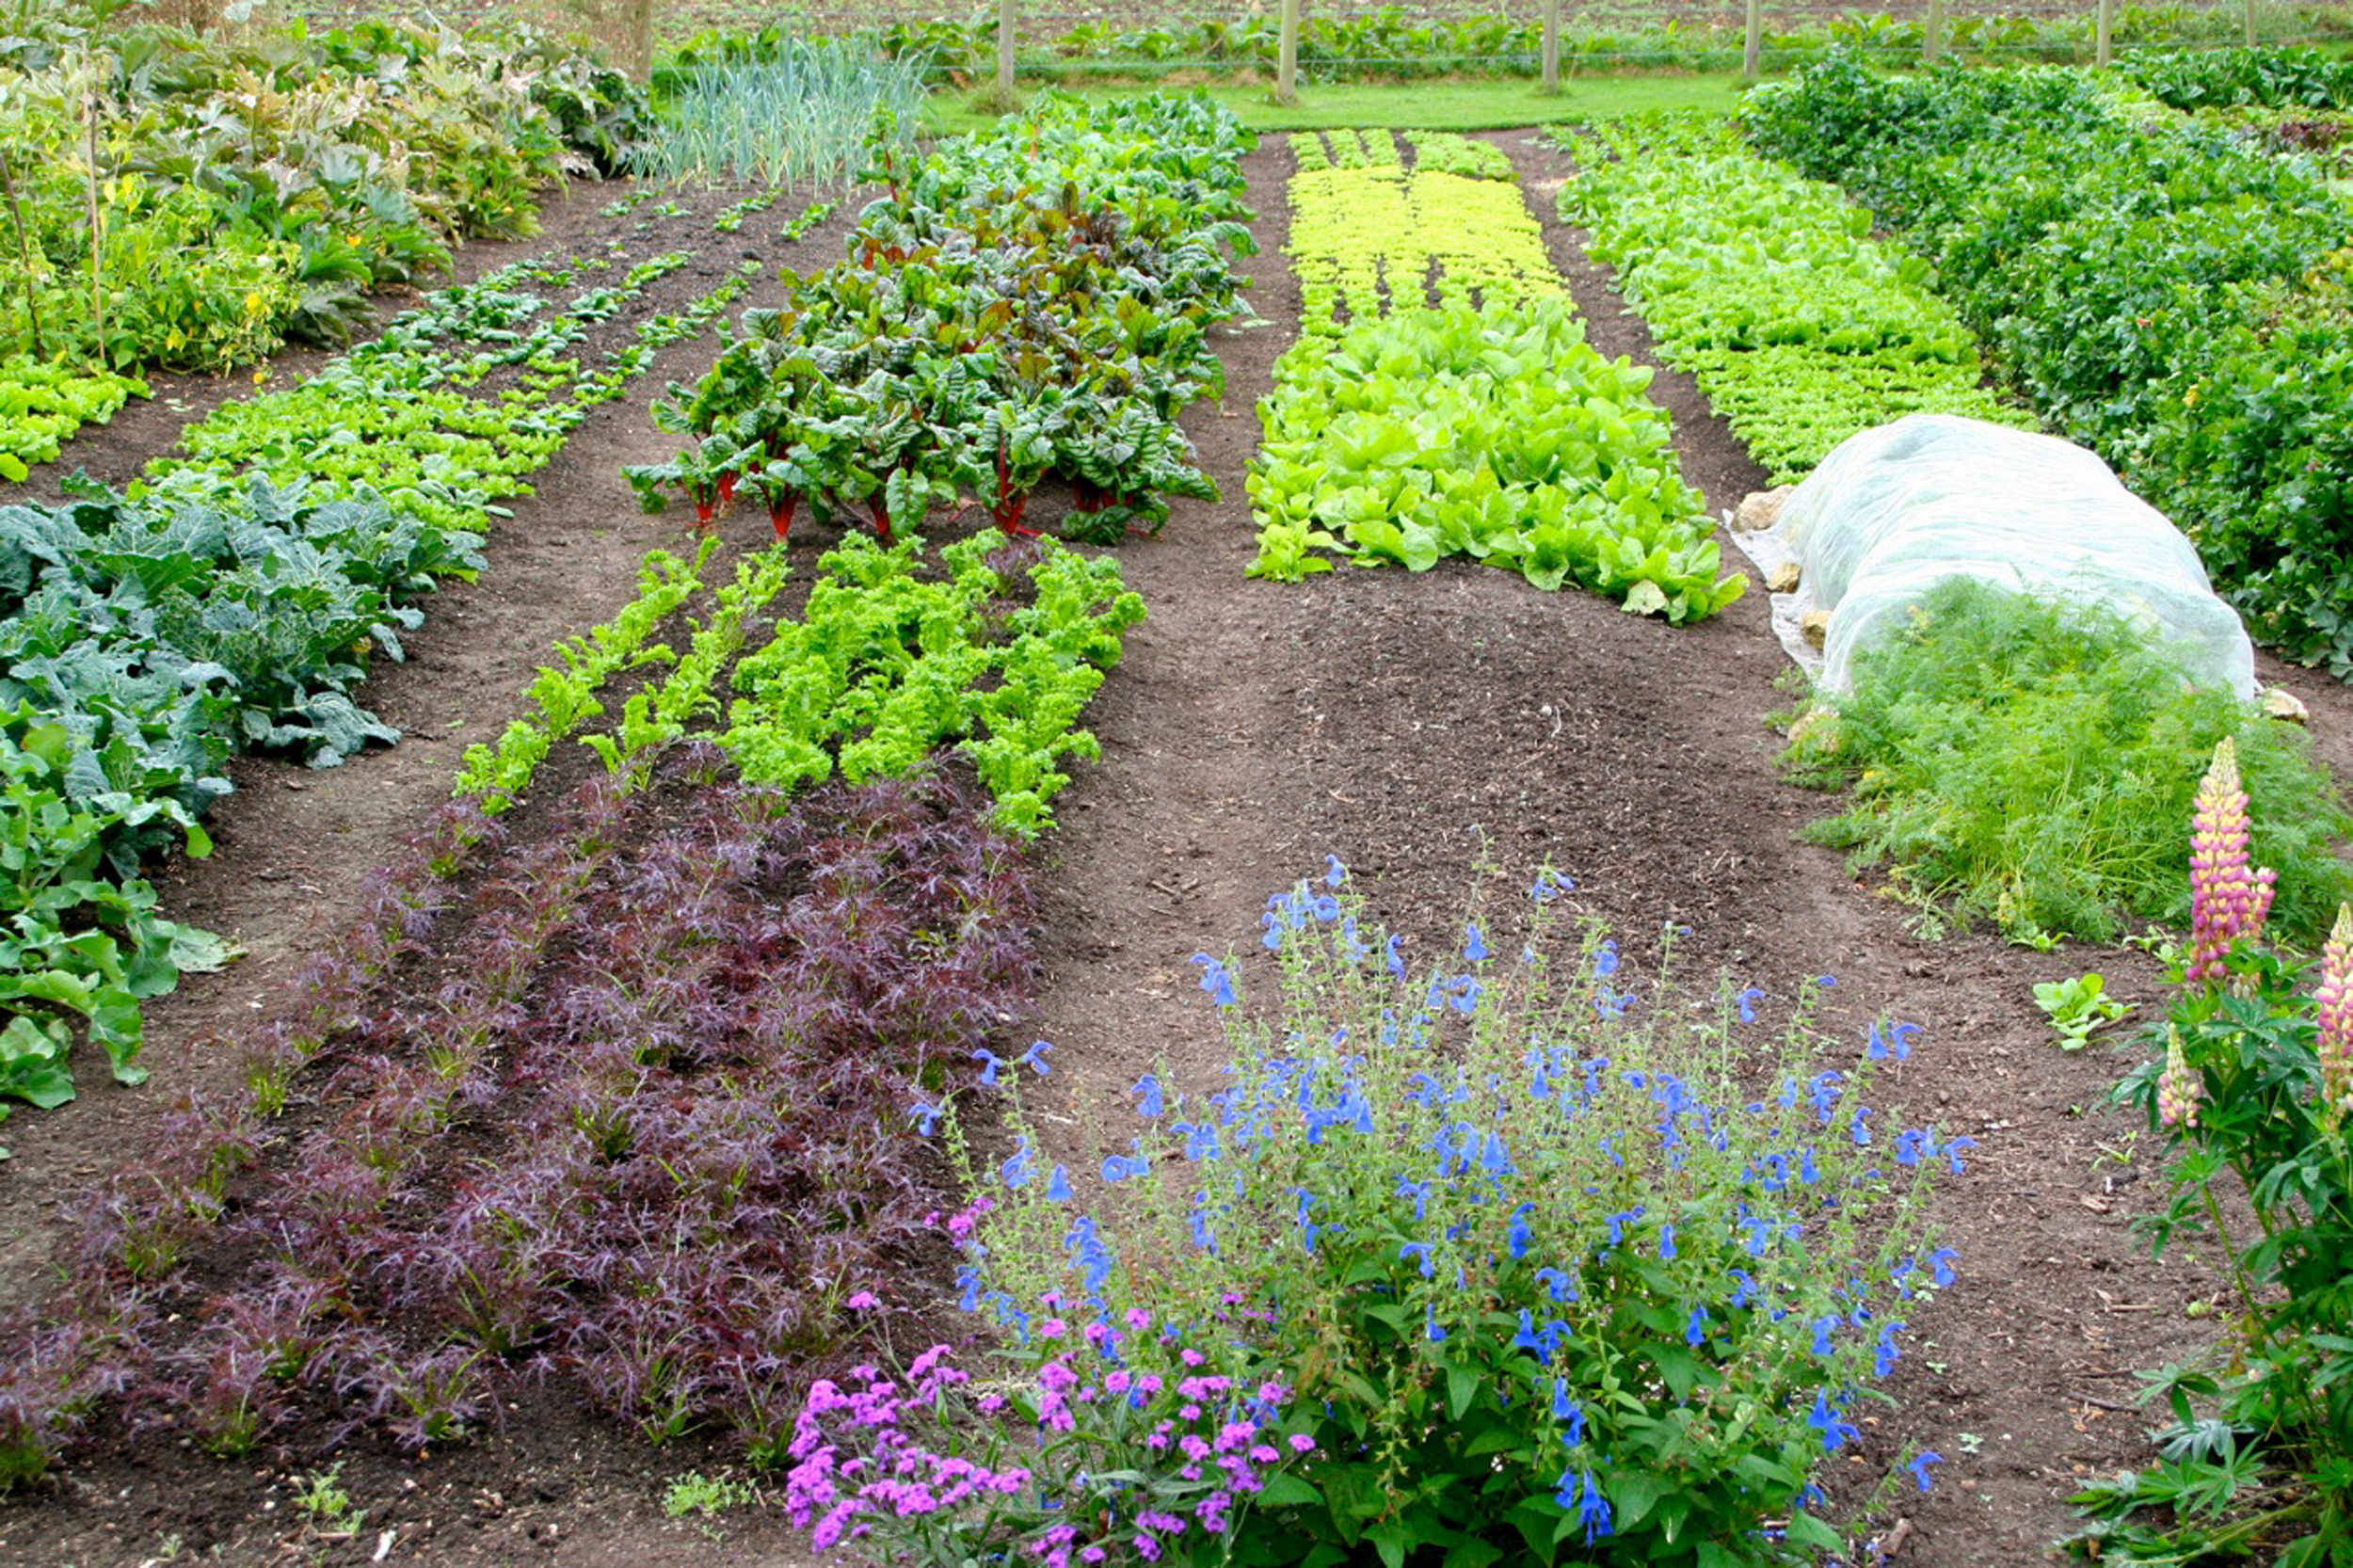
\includegraphics[width=0.6\textwidth]{images/beds.jpg}
    \caption{Beds in a market garden}
    \label{fig:beds}
\end{figure}

\paragraph{Crop rotation} In order to preserve the soil from draining and to eliminate some diseases specific to some plant species, some market gardener rotate their cropping. If they plant one type of vegetable on a bed, the year after they will plant another type of vegetable on this bed. They will not plant two years in a row the same vegetable on the same bed.

\section{Daily life scenario}

\paragraph{Seasons} Market gardeners live by the rhythm of the seasons: they have a peak of work during the Spring and the Summer. Harvests continue during Autumn but during Winter they usually have less things to do in the garden. 

\paragraph{Planning}

Most gardeners plan their cropping during winter\cite{planification-methodology}, when they have more time to think about what they want to grow this year. Planning the coming year has several advantages : 

\begin{itemize}
	\item Know in advance what amounts of seeds and fertilizers they will have to order
	\item Take the time to decide what to grow and in what quantities
	\item Look back at the previous year to see which vegetables were the most profitable and adjust cropping according to this experience.
	\item Gain time during the rush season by having clearly in mind what has to be done
	\item Organise the year to spread the work as most as possible (everything can not be seeded the same week)
\end{itemize}

While really useful, this planning part is not always done by market gardeners. 

\paragraph{Adaptations}
Once the work season has started, this planning has to be adapted to the reality on the ground.
The weather is the major factor of changes in the planning. Indeed, some seeding requires several days of dry weather followed by one day of rain for example. In the case of difficult weather (late frost, large humidity,...), whatever was the initial plan, the gardener will have to adapt his schedule to the weather.
Others factors that disrupt the work set-up can be diseases in the crops, short staffing or hardware issues.
One example scenario could be:
We are the first week of July, the season is in full swing. Tim is a market gardener and had planned to plant endives this week. The weather conditions are perfect, so he could stick to his plan. Unfortunately, his tomatoes have mildew\footnote{an epidemic fungus  \url{https://en.wikipedia.org/wiki/Mildew}} and if he wants to save his tomatoes' crops, he has to treat them immediately.

This example shows that some events have priority over the initial plan and confirm the idea that initial planning is meant to evolve.

It is essential for a market garden to be able to adapt its plans to a specific situation and to keep a clear head as we go along the season. Planning is already not and easy task, but adapting to changes is even harder. 



\section{Profitability of market gardens}


% These antoinette dumont
%\begin{itemize}
%\item difficile d'estimer les couts unitaires:
%\item difficile d'estimer combien rapporte chaque légume
%\item difficile de savoir combien de temps passer sur chaque culture et donc de savoir laquelle est la plus profitable.
%\end{itemize}
%
%
%


\paragraph{Workforce} Market gardeners don't count their hours as regular workers. They work all day in order to reach their objectives of the day. Most of them have no idea of how long each culture takes. It also means that they have no idea how profitable their cultures are. Moreover, they often need external workers to help them during the peak season. These external workers represent 50\% of productions costs \cite{fortier}. Consequently, organizing the work to reduce the need of external workers can have a considerable impact on the garden's profitability.

\paragraph{Vegetables profitability}
Some vegetables are more profitable than others. For example, Jean-Martin Fortier \cite{fortier} in his book gives data about the profitability of the vegetables he's growing. However, most farmer don't do this analysis on their production and have therefore, no idea of which cropping is the most profitable. Even in the table of Jean-Martin Fortier, we have no idea of the work time needed for each culture. And yet we have seen before that workforce represent a significant cost.
Moreover, from one area to another it is reasonable to think that some crops will be more profitable than others. Depending on the clients' preferences or the soil type, some vegetables will be easier to sell or to crop.
Gardeners are mostly not analysts and don't have the right tools to give them an idea of how profitable their business is and how they could be more efficient.

\paragraph{Others profitability factors}

\begin{itemize}
\item Retail strategy: different retails strategies will give different revenues, the more intermediaries there are between the producer and the client, the less the producer will gain.
\item Pricing strategy: of course, the selling price of vegetables will affect the profitability of this vegetables. Depending on which retail strategy is chosen, prices will be more or less flexible.
\end{itemize}

Antoinette Dumont has dedicated her doctoral thesis on the subject of market gardens' profitability.\cite{adumont}

\section{Researches in gardening}

\todo[inline]{Complete this section}

\section{Existing tools}

From our researches, there is not a lot of software to help farmers of all kind in their daily life. Furthermore, most of them are not open source.

First, we found software like \emph{Mes petits légumes}\cite{mespetitslegumes} intended for non-professional market gardeners, with a great library of data about lots of vegetables. The software can be bought once for 19 \euro{} or one can use the free incomplete version. Two screenshots of this application are shown on image \ref{fig:mespetitslegumes}

\begin{figure}
\centering
\begin{subfigure}{.5\textwidth}
  \centering
  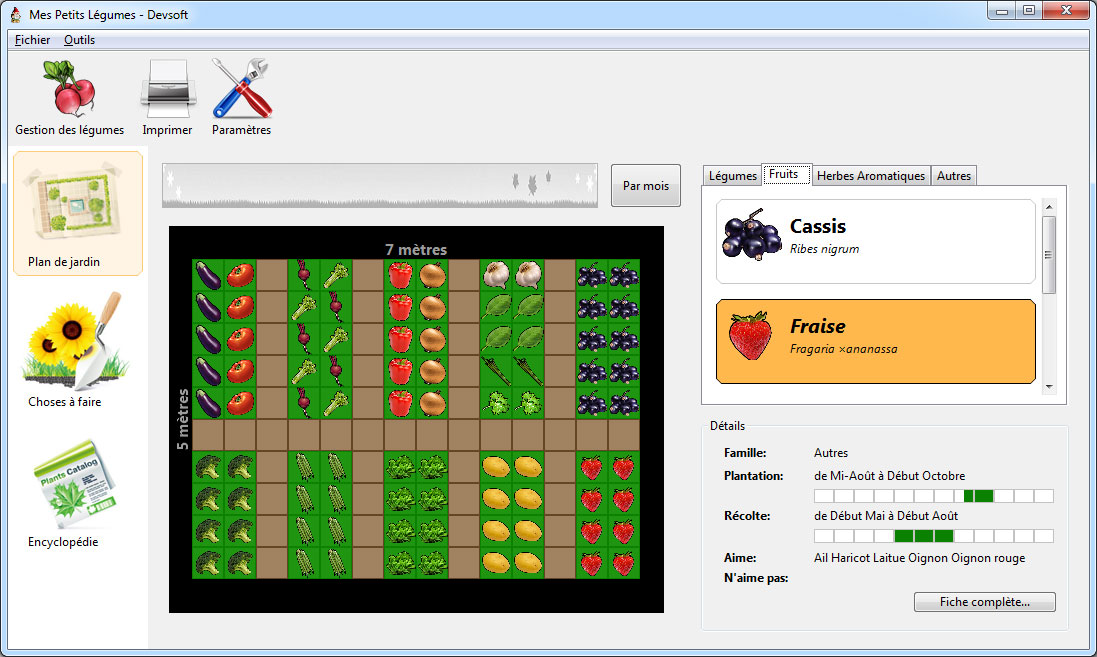
\includegraphics[width=0.9\linewidth]{images/petitslegumes1.jpg}
  \caption{Visual representation of a garden planning}
  \label{fig:petitslegumes1}
\end{subfigure}%
\begin{subfigure}{.5\textwidth}
  \centering
  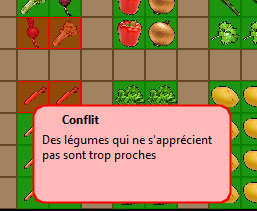
\includegraphics[width=0.7\linewidth]{images/petitslegumes2.jpg}
  \caption{Intercropping advices}
  \label{fig:petitslegumes2}
\end{subfigure}
\caption{Screenshots of the software \emph{Mes petits légumes}}
\label{fig:mespetitslegumes}
\end{figure}



Then, we have softwares like \emph{LEA}\cite{lea-agri} more focused on the management of the business and intended for big farms. It can generate bill from tractor work. It helps managing stocks and uses of fertilizers. 
Once again, the software is not open source and a subscription is required to use it.

Finally, we have found a software that seems to have a purpose and a target audience similar to this project. \emph{Tend}\cite{tend} is a software developed in the USA by a Startup. It has lots of features, including a databases of vegetables, a task calendar and an expenses section. The main feature (constitute a crop plan by adding plantings) is shown on figure \ref{fig:tend}.

\begin{figure}
\centering
\begin{subfigure}{.5\textwidth}
  \centering
  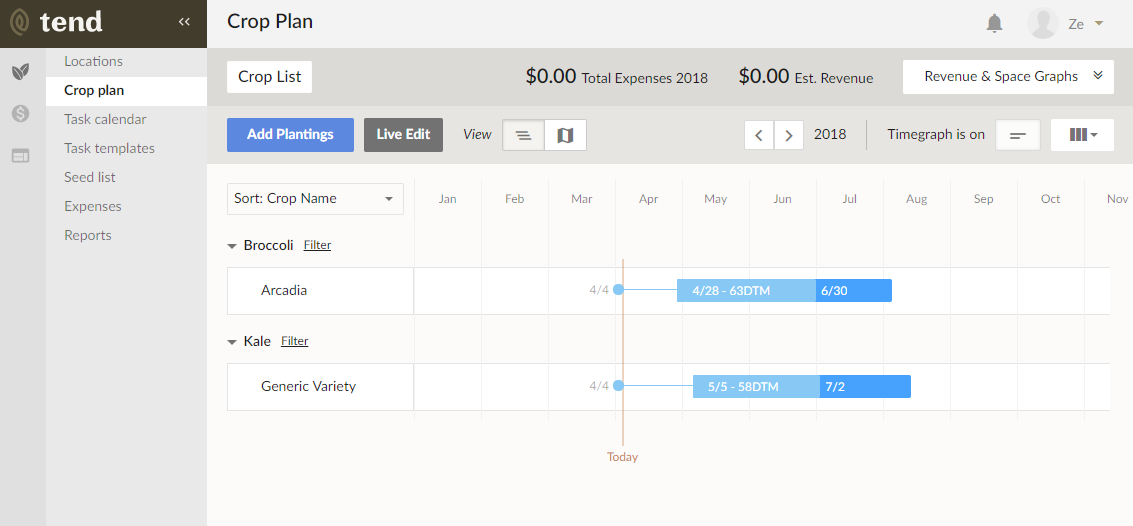
\includegraphics[width=0.9\linewidth]{images/tend1.PNG}
  \caption{Planning view}
\end{subfigure}%
\begin{subfigure}{.5\textwidth}
  \centering
  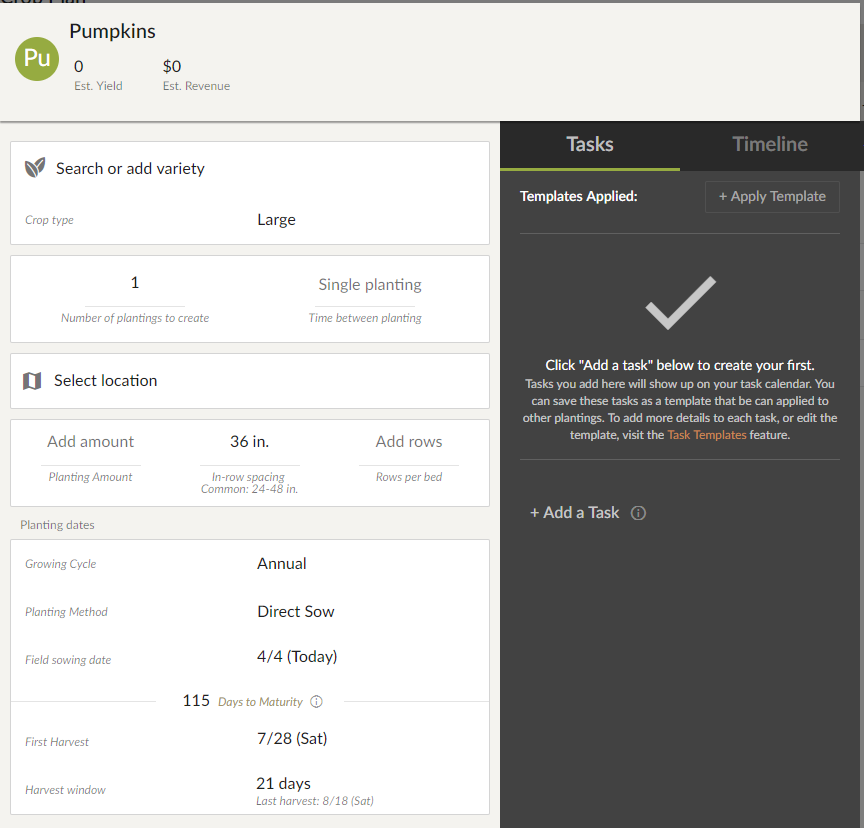
\includegraphics[width=0.7\linewidth]{images/tend2.PNG}
  \caption{Adding a new plantation}
\end{subfigure}
\caption{Screenshots of the software \emph{Mes petits légumes}}
\label{fig:tend}
\end{figure}

These software show that farmers are in need of tools to help them in their planning and management. The poorness of software really adapted to their needs show that this field has been forgotten by technology.


\section{Conclusion}

From this analysis of the field of market gardening, 
\todo[inline]{+ say that this is where this thesis comes in}